%label:"exm:contactManifold"
%author:JeffHicks
%name:"contact hypersurfaces"
%type:"example"
%parent:def:contactManifold


    A key set of examples of contact manifolds come as hypersurfaces of symplectic manifolds. Let $(X, \omega)$ be a symplectic manifold. Suppose that there is an expanding vector field $Z$ on $X$, that is, a vector field so that 
    \[\mathcal L_Z \omega = \omega.\]
    The symplectic manifold $X$ is exact, with primitive given by $\lambda=\iota_Z \omega$.
    Let $i:M\into  X$ be a hypersurface which is transverse to $Z$. Then the restriction $\alpha:=\lambda|_M$ is an example of a contact form. We see that the form  
    \begin{align*}
        \alpha \wedge d\alpha^{n-1} =& i^* (\iota_Z \omega \wedge \omega^{n-1})\\
    \end{align*}
    is nonvanishing, as $\omega^n$ is a volume form and $Z$ is transverse to $M$.

    The simplest example to consider come from $\CC^n= \RR^{2n}$, where the radial vector field $Z=\frac{1}{2}\sum_i \left(x_i \partial_{x_i} + y_i\partial_{y_i}\right)$ provides an example of an expanding vector field. The associated primitive for the symplectic form is 
    \[\iota_Z \omega =\sum_{i=1}^n x_i dy_i-y_idx_i \]
     This radial vector field plays especially nicely with respect to the moment map, 
    \begin{align*}
        p: \RR^{2n}\to& (\RR_{\geq 0})^n\\
            (x_i, y_i)\mapsto&\frac{1}{2} (x_i^2+y_i^2)
    \end{align*}
    We give the base of the moment polytope $(\RR_{\geq 0})^n$ coordinates $(p_1, \ldots, p_n$).  
    At every point $(x_i, y_i)\in \RR^{2n}$, we can project the Liouville vector field to 
    \[p_*Z_{(x_i, y_i)}= \sum_{i=1}^n (x_i^2+y_i^2) \partial_{p_i} =\frac{1}{2}\sum_{i=1}^n  p_i \partial_{p_i}.\]
    In particular, if we have a hypersurface $N\subset (\RR_{\geq 0})^n$ which is transverse to the radial vector field $\sum_{i=1}^n  p_i \partial_{p_i}$ and whose preimage $M:=p^{-1}(N)\subset \RR^{2n}$ is a smooth hypersurface, then  $M$ is a contact manifold.
    \label{exm:contactManifold}
    %tag:000X
%label:fig:liuvilleMomentMapR2
%author:JeffHicks
%name:"Liouville structure on $\CC^2$ as viewed from the moment map"
%type:figure
%parent:exm:contactManifold
%caption:"The Liouville structure on $\CC^2$ as viewed from the moment map"


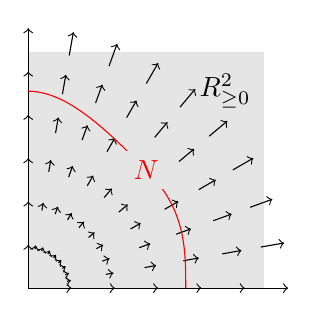
\begin{tikzpicture}
    \fill[gray!20] (0,0)--(3, 0)--(3,3)--(0,3)--cycle;
    \draw (0,0)--(3,0) (0,3)--(0,0);
    \foreach \r in { .5, 1,1.5, 2,2.5, 3} {
        \foreach \t in {0,...,9} {
            \draw[->] ({\r * cos(10*\t)},{ \r * sin(10*\t) })-- ({1.1*\r * cos(10*\t)},{ 1.1*\r * sin(10*\t) });
            }
    }
    
    \draw[red] (0,2.5) .. controls (0.5,2.5) and (1,2) .. (1.5,1.5) node[fill=gray!20] {$N$} .. controls (2,1) and (2,0.5) .. (2,0);
    \node at (2.5, 2.5) {$\mathbb R_{\geq 0}^2$};
    \end{tikzpicture}
